\documentclass[12pt]{article}
\usepackage[utf8]{inputenc}
\usepackage[T1]{fontenc}
\usepackage[czech]{babel}
\usepackage[margin=1.8cm]{geometry}
\usepackage{graphicx}
\usepackage{hyperref}
\usepackage{parskip}
\usepackage{float}
\usepackage{xurl}

\hypersetup{
  hidelinks,
  pdfauthor={Dominik Honza xhonza04},
  pdftitle={Automatické počítání skóre ve hře šipky}
}

\setlength{\parindent}{0pt}
\newcommand{\docsection}[1]{\section*{#1}\addcontentsline{toc}{section}{#1}}

\begin{document}

\begin{titlepage}
\centering
\vspace*{2.5cm}
{\Huge \textbf{Automatické počítání skóre ve hře šipky s využitím Raspberry Pi 4B}\par}
\vspace{1.5cm}
{\Large Technická dokumentace projektu\par}
\vspace{1.2cm}
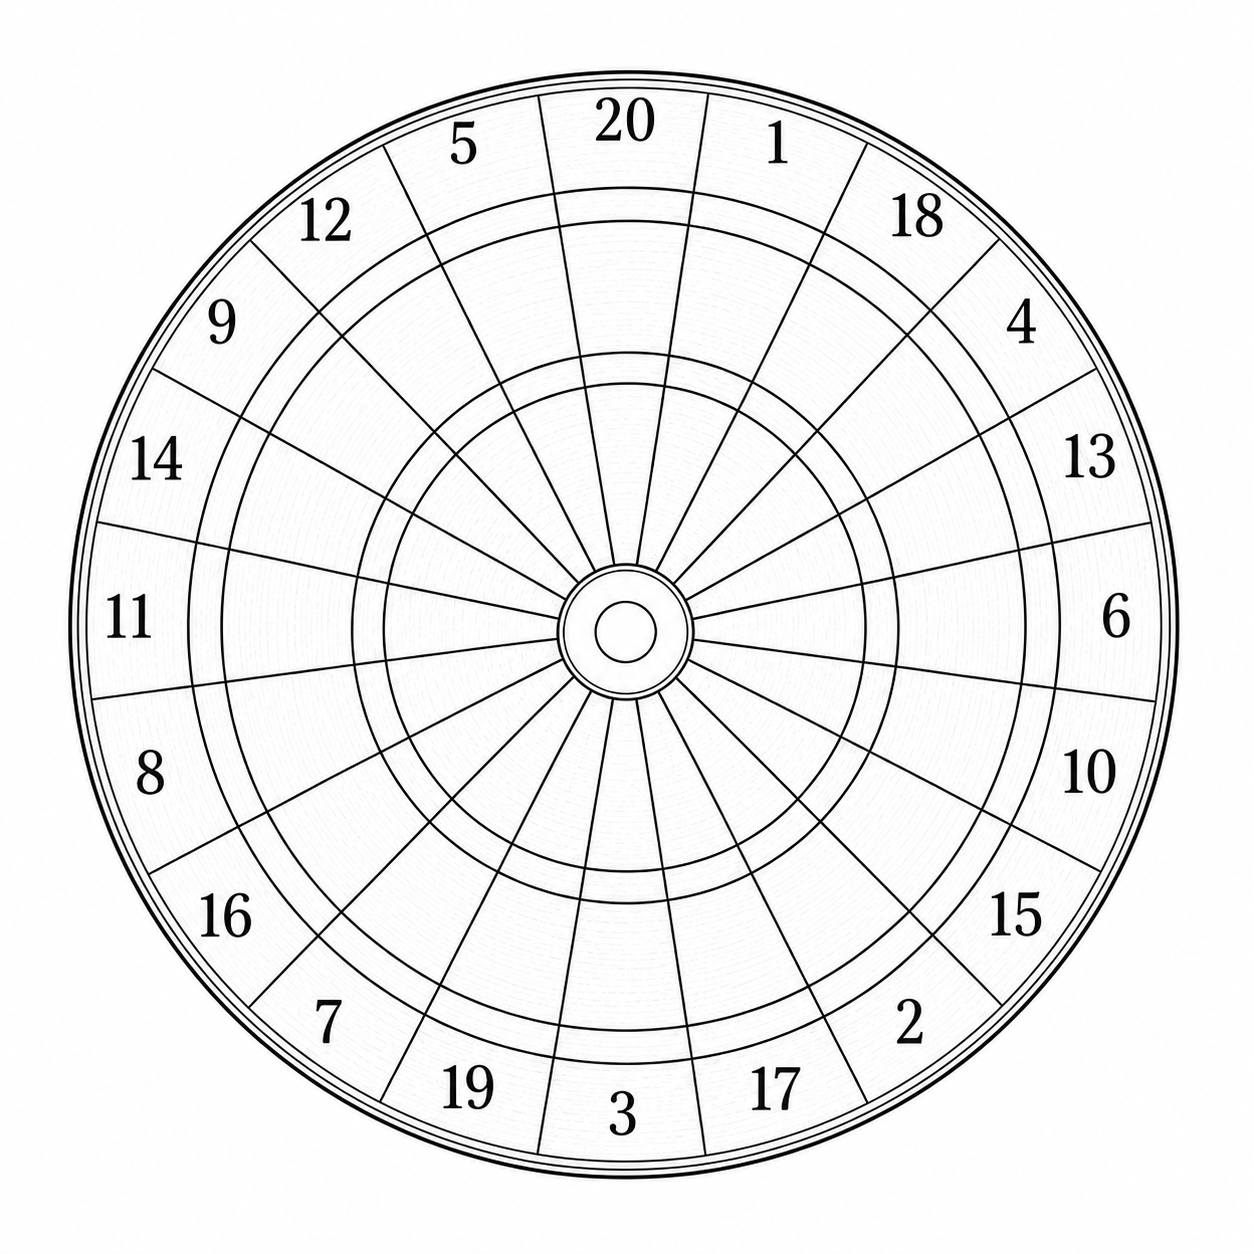
\includegraphics[width=7cm,keepaspectratio]{Target.png}\par
\vspace{1.2cm}
\vfill
{\Large Autor: Dominik Honza xhonza04\par}
\vspace{0.4cm}
{\Large Místo: Brno, FIT VUT\par}
\vspace{0.4cm}
{\Large Datum: 1. 5. 2026\par}
\vspace*{2cm}
\end{titlepage}

\tableofcontents
\clearpage

\docsection{Popis projektu}

Cílem projektu je návrh a realizace systému pro automatické skórování při hře šipky. Systém využívá USB kameru pro snímání terče, následné zpracování obrazu a automatický výpočet bodového zisku podle místa zásahu šipky. Výsledky jsou zobrazovány na dotykovém LCD displeji, který zároveň slouží jako jednoduché uživatelské rozhraní.

Projekt demonstruje možnosti využití platformy Raspberry Pi v oblasti:

\begin{itemize}
\item zpracování obrazu
\item detekce objektů
\item výpočtu skóre podle pozice zásahu
\item realizace interaktivního uživatelského rozhraní
\end{itemize}

\docsection{Cíl řešení}

Základní princip systému spočívá v tom, že prostor před terčem je průběžně snímán USB kamerou. Raspberry Pi 4 Model B analyzuje obraz pomocí algoritmů počítačového vidění a identifikuje pozici zásahu šipky. Na základě této pozice systém:

\begin{itemize}
\item určí sektor terče
\item rozliší single, double a triple
\item rozpozná bull a outer bull
\item vypočítá odpovídající bodovou hodnotu
\end{itemize}

Zpracované informace jsou zobrazovány na dotykovém displeji \href{https://rpishop.cz/lcd-oled-displeje-hat/1203-waveshare-35-lcd-b-displej-320480-dotykovy-rezistivni.html?msclkid=4a6799ecda6f1137f7b9f0184b84918c}{Waveshare 3.5" LCD B 320x480 s rezistivní dotykovou vrstvou}, který slouží zejména pro:

\begin{itemize}
\item zobrazování aktuálního skóre
\item přehled hráčů
\item indikaci průběhu tahu
\item jednoduché ovládání herních funkcí
\end{itemize}

\clearpage
\docsection{Použitý hardware a software}

Řešení v této složce předpokládá následující sestavu:

\begin{itemize}
\item Raspberry Pi 4 Model B
\item USB kamera Canyon CWC3 3 Megapixel USB 2.0 s mikrofonem
\item dotykový displej \href{https://rpishop.cz/lcd-oled-displeje-hat/1203-waveshare-35-lcd-b-displej-320480-dotykovy-rezistivni.html?msclkid=4a6799ecda6f1137f7b9f0184b84918c}{Waveshare 3.5" LCD B 320x480} připojený jako framebuffer \texttt{/dev/fb1}
\item dotykový vstup dostupný přes \texttt{/dev/input/event0}
\item lokální síť pro MJPEG náhled
\end{itemize}

Použité knihovny a technologie:

\begin{itemize}
\item Python 3
\item OpenCV (\texttt{cv2})
\item NumPy
\item \texttt{evdev}
\end{itemize}

Typická instalace Python balíčků:

\begin{verbatim}
pip install opencv-python numpy evdev
\end{verbatim}

\docsection{Struktura řešení}

Implementace je rozdělena do několika částí:

\begin{itemize}
\item \texttt{main.py} řídí hlavní běh aplikace, hráče, snímání kamery a přepínání tahů
\item \texttt{dart\_detector.py} vyhledává změny v obraze, kontury a odhaduje špičku šipky
\item \texttt{warp.py} provádí perspektivní transformaci a převod zásahu do normalizovaného prostoru terče
\item \texttt{enumerate\_score.py} obsahuje logiku výpočtu skóre podle sektoru a vzdálenosti od středu
\item \texttt{display.py} vykresluje skóre a stav hry na LCD displej
\item \texttt{stream\_server.py} zpřístupňuje zpracovaný obraz jako MJPEG stream
\item \texttt{touch\_input.py} obsluhuje dotykový vstup
\item \texttt{calibration.json} ukládá kalibrační body a úhel natočení terče
\item \texttt{CalibrationGUI/} obsahuje samostatné grafické rozhraní pro kalibraci terče a ladění transformačních bodů
\end{itemize}

\clearpage
\docsection{Princip realizace}

Zpracování obrazu v jednokamerové verzi probíhá v několika krocích:

\begin{enumerate}
\item Inicializace kamery. \texttt{main.py} otevře \texttt{/dev/video0} přes OpenCV, nastaví rozlišení \texttt{1280x720} a počká na ustálení expozice.
\item Vytvoření referenčního snímku. Systém pořídí několik snímků prázdného terče, zprůměruje je a uloží jako stabilní referenční obraz \texttt{frame.jpg}.
\item Snímání aktuálního stavu. Během hry je průběžně získáván nový snímek z kamery.
\item Detekce změny v obraze. \texttt{dart\_detector.py} porovnává aktuální rozmazaný šedotónový snímek s referenčním snímkem pomocí \texttt{cv2.absdiff()}.
\item Odhad špičky šipky. Pro každou nalezenou konturu se spočítá její centroid a jako odhad špičky šipky se vybere bod kontury nejvzdálenější od centroidu.
\item Perspektivní transformace. \texttt{warp.py} načte kalibrační body terče a převede zásah z perspektivního pohledu kamery do normalizovaného pohledu shora.
\item Výpočet skóre. Ve znormalizovaném prostoru se z polohy zásahu určí prstenec a sektor, z nichž se vypočítá výsledná bodová hodnota.
\item Zobrazení výsledku. Skóre je zobrazeno na LCD displeji a zpracovaný snímek je současně dostupný přes MJPEG stream.
\end{enumerate}

Schéma celé pipeline je shrnuto na následujícím diagramu:

\begin{center}
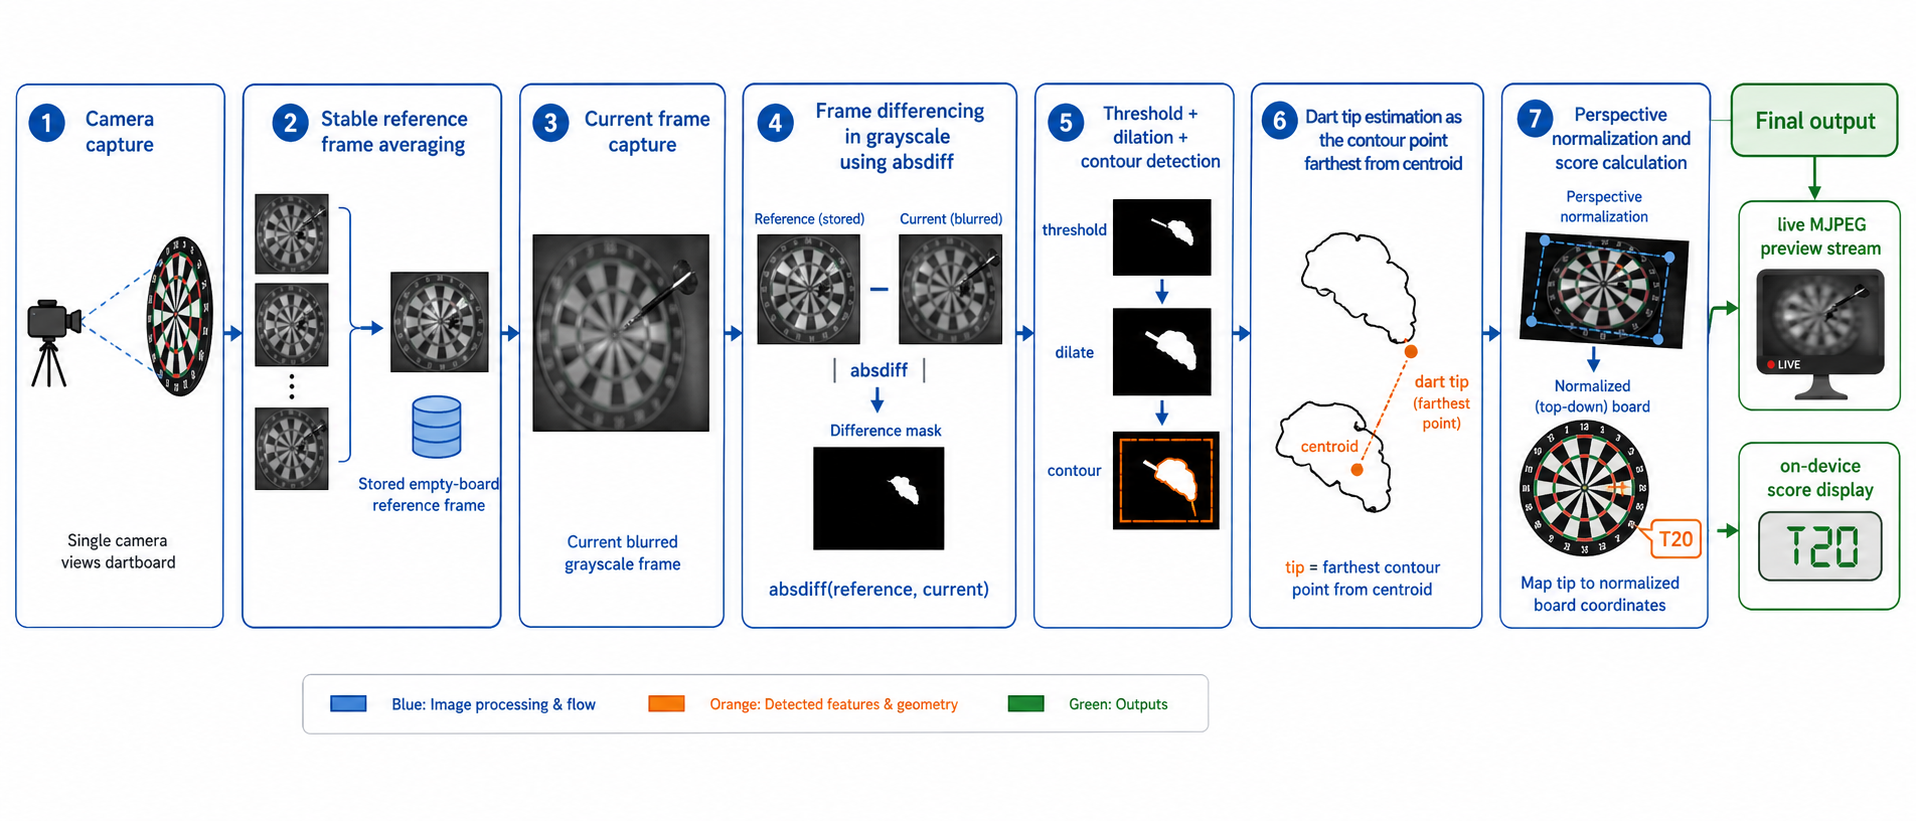
\includegraphics[width=\linewidth,keepaspectratio]{Diagram.png}
\end{center}

\clearpage
\docsection{Detekce zásahu}

Detektor pracuje na principu rozdílu mezi referenčním obrazem prázdného terče a aktuálním snímkem. V praxi to znamená, že nové objekty v obraze, typicky šipka zapíchnutá v terči, vytvoří viditelnou změnu. Po nalezení kontur systém:

\begin{itemize}
\item odfiltruje příliš malé oblasti
\item spočítá obdélník ohraničující zásah
\item vyznačí konturu
\item určí směr od centroidu ke špičce
\item zobrazí rozpoznané skóre přímo do náhledu
\end{itemize}

Následující obrázky ukazují typické výstupy detekce:

\begin{center}
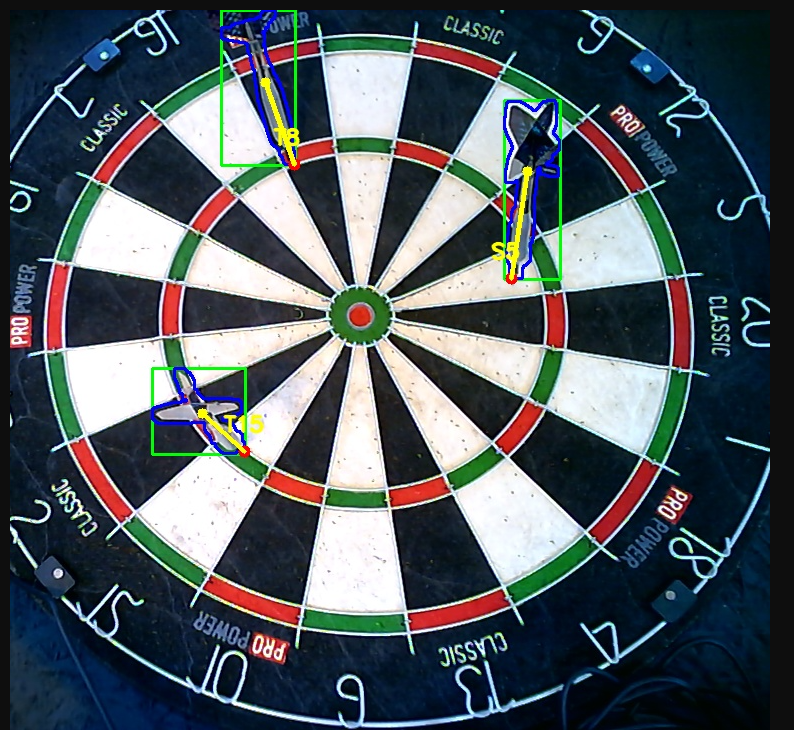
\includegraphics[height=7cm,keepaspectratio]{TargetHit.png}
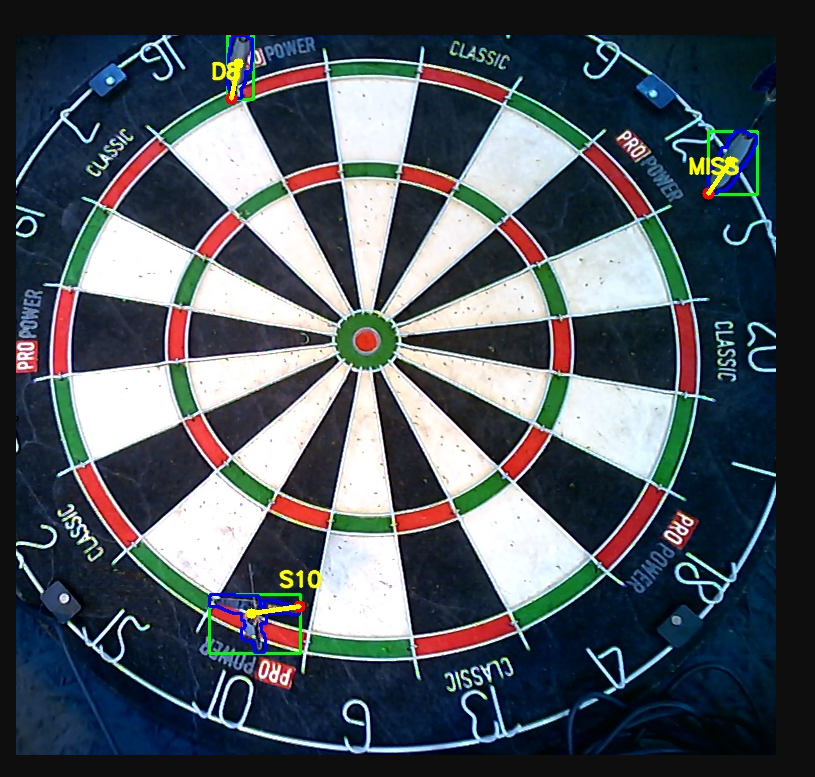
\includegraphics[height=7cm,keepaspectratio]{TargetMiss.png}
\end{center}

\docsection{Kalibrace a perspektivní transformace}

Aby bylo možné správně určit polohu zásahu, je nutné převést perspektivní pohled kamery na normalizovaný model terče. Tento převod je řízen hodnotami v souboru \texttt{calibration.json}.

Význam položek:

\begin{itemize}
\item \texttt{tl}, \texttt{tr}, \texttt{br}, \texttt{bl} určují čtyři kalibrační body použité pro perspektivní transformaci
\item \texttt{angle} upravuje natočení sektorů v transformovaném obrazu
\item \texttt{center} je zachován kvůli kompatibilitě s kalibračními nástroji
\item \texttt{score\_angle} lze volitelně použít pro jemné doladění mapování sektorů
\end{itemize}

Kalibrační nástroj umožňuje měnit body a okamžitě kontrolovat, zda zarovnání sektorů a kružnic odpovídá reálnému terči.

Součástí projektu je také samostatná složka \texttt{CalibrationGUI/}, která obsahuje dedikované Calibration GUI pro pohodlné nastavování kalibračních bodů a ověřování perspektivní transformace mimo hlavní běh aplikace.

\begin{center}
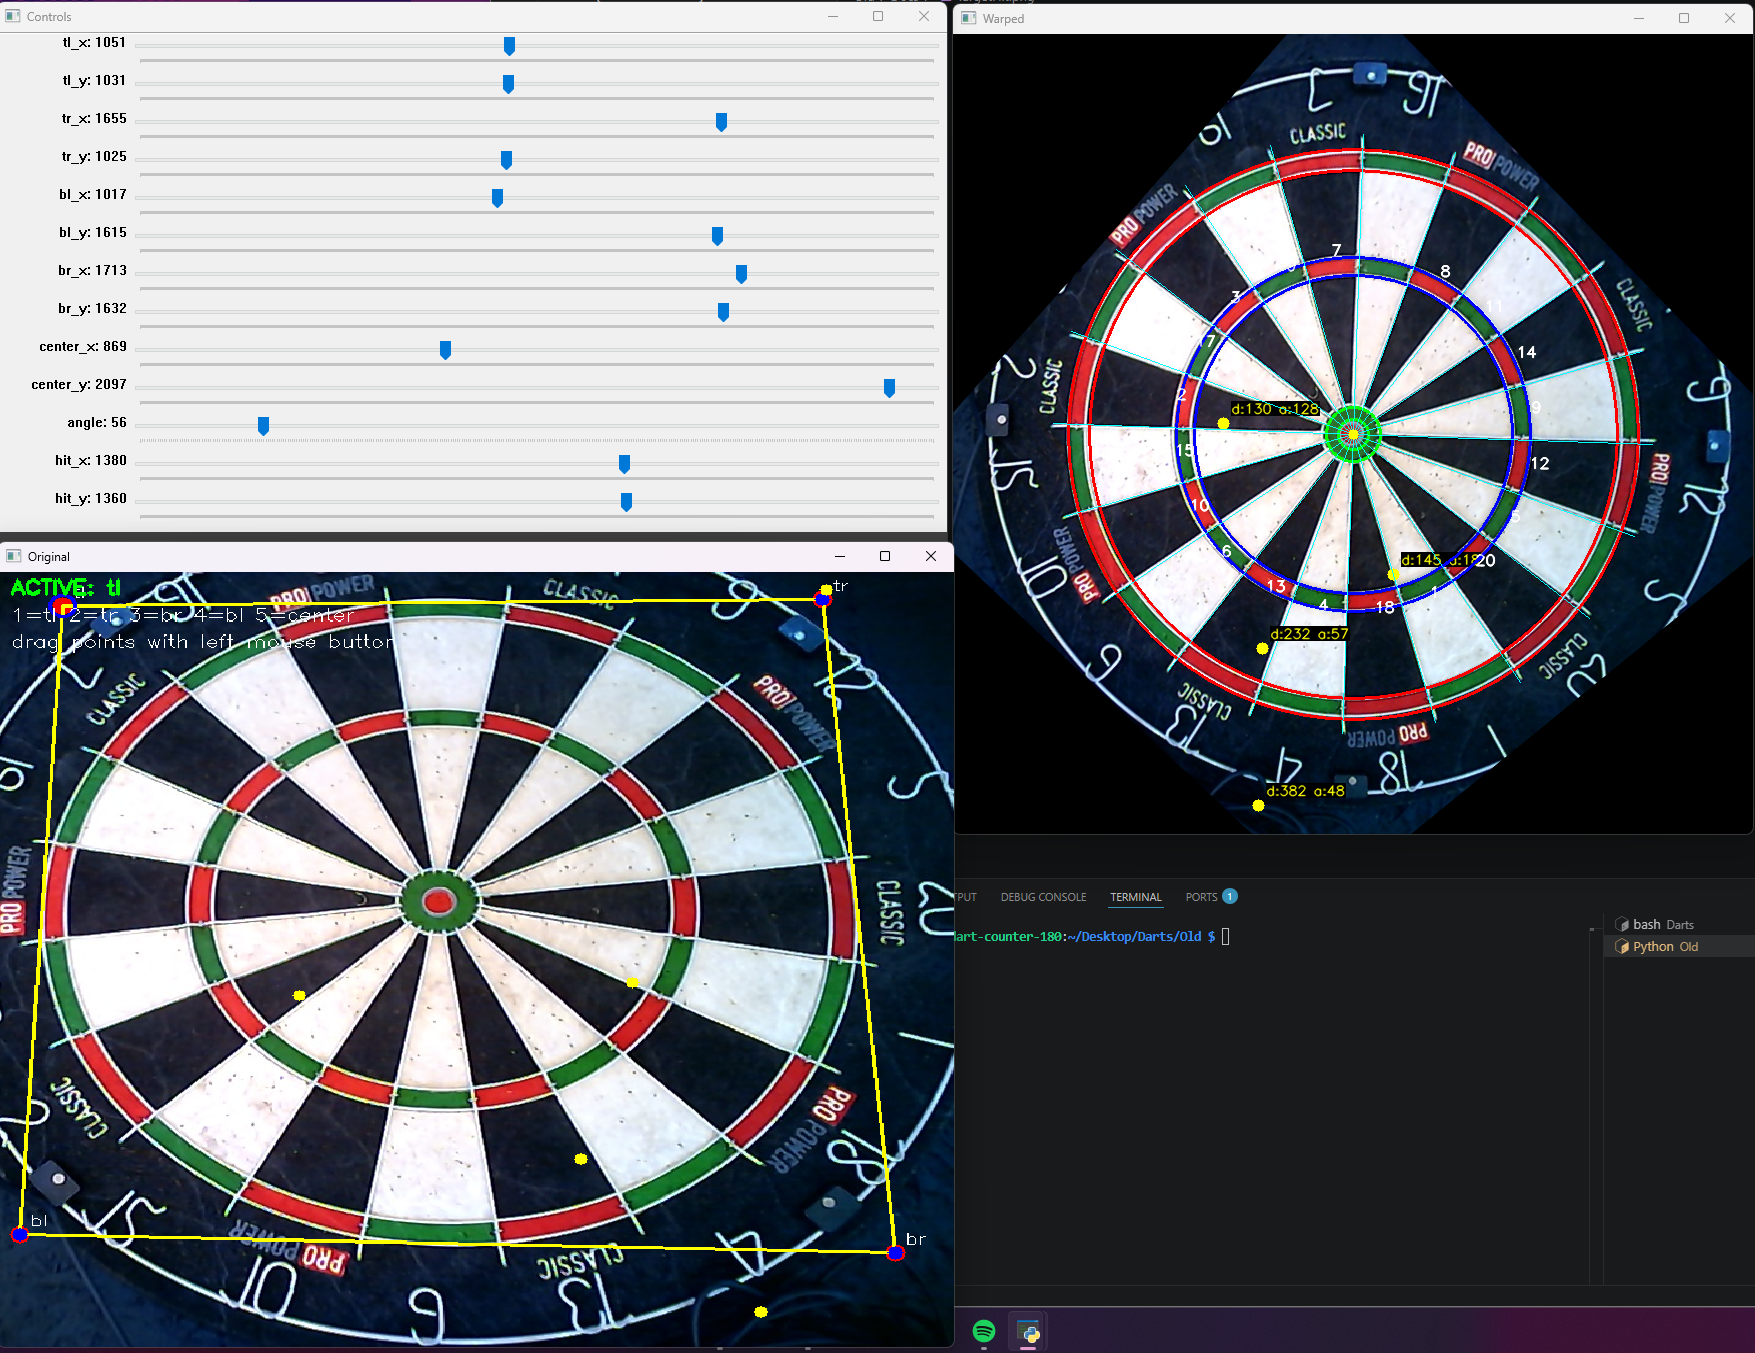
\includegraphics[width=15.5cm,keepaspectratio]{CalibrationTool.png}
\end{center}

Následující diagram ilustruje samotný princip perspektivní transformace, tedy převod zásahu z pohledu kamery do jednotného normalizovaného prostoru terče:

\begin{center}
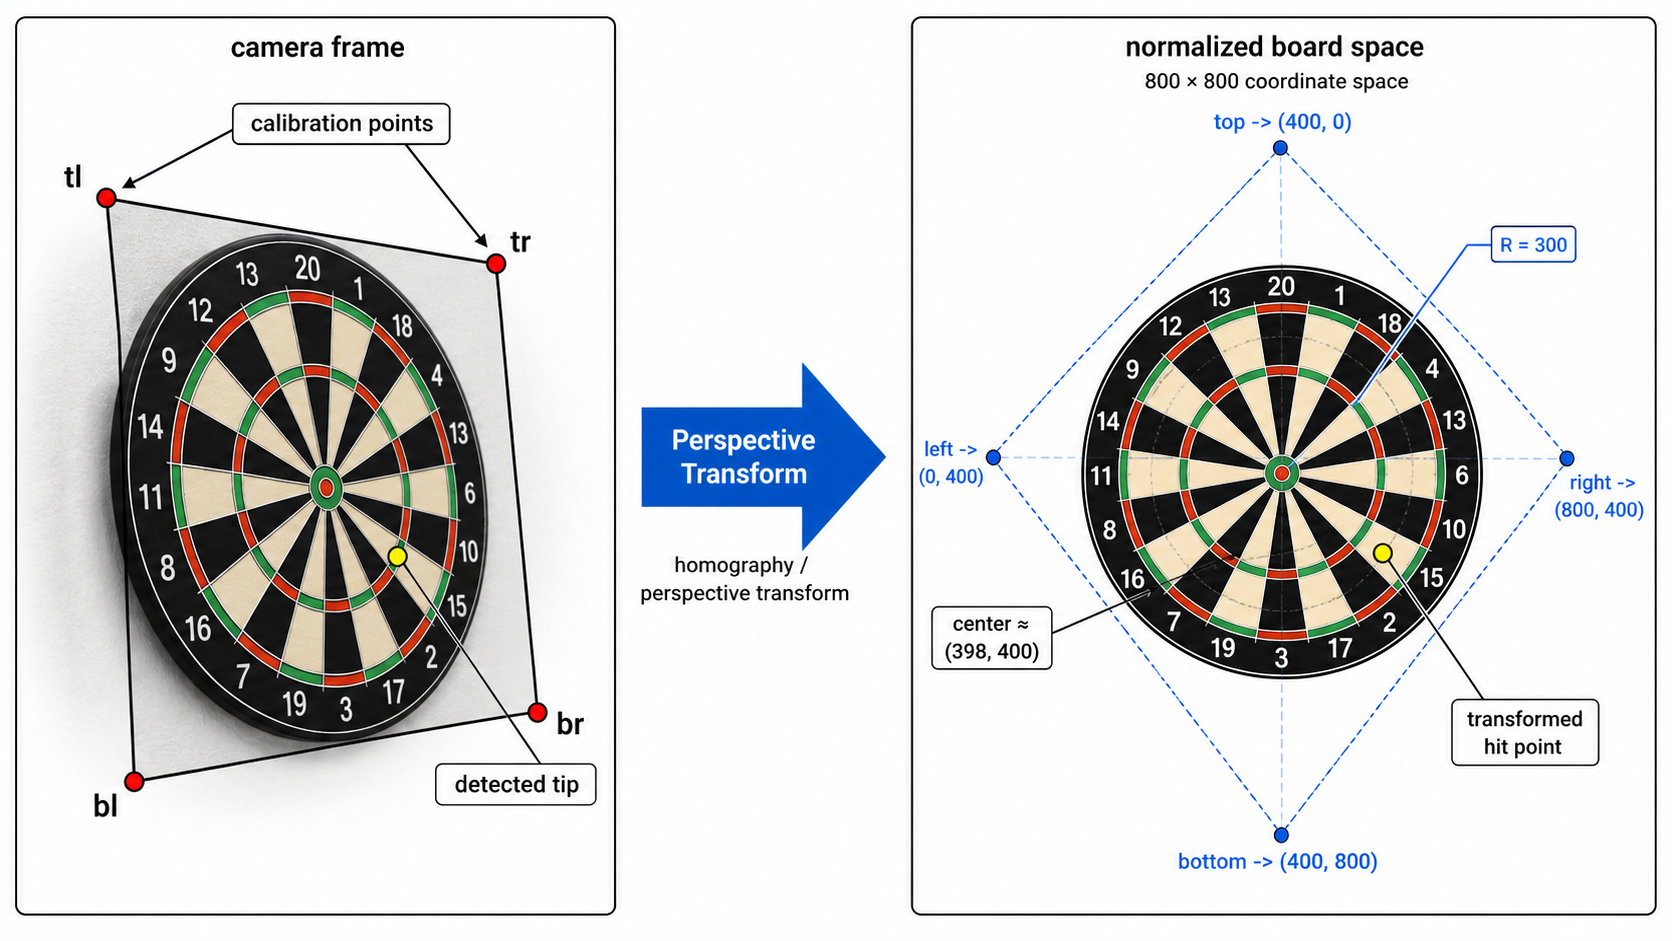
\includegraphics[width=15.5cm,keepaspectratio]{PerspectiveTransform.png}
\end{center}

\clearpage
\docsection{Výpočet skóre}

Po perspektivní transformaci systém pracuje s normalizovaným terčem o velikosti \texttt{800x800} pixelů. Skóre je určeno kombinací:
vzdálenosti zásahu od středu terče a úhlu zásahu vůči středu.

Logika odpovídá souboru \texttt{enumerate\_score.py}:

\begin{itemize}
\item \texttt{BULL} a \texttt{OUTER\_BULL} pro zásah do středu
\item \texttt{TRIPLE} pro trojitou kružnici
\item \texttt{DOUBLE} pro dvojitou kružnici
\item \texttt{SINGLE} pro běžná pole uvnitř terče
\item \texttt{MISS} mimo bodovanou oblast
\end{itemize}

Sektor se určí z úhlu vektoru mezi středem a transformovaným bodem zásahu. Výsledná hodnota skóre vznikne spojením typu prstence a čísla sektoru. Následující diagram ukazuje, jak je zásah převeden do normalizovaného prostoru terče a jak z této pozice vznikne finální skóre:

\begin{center}
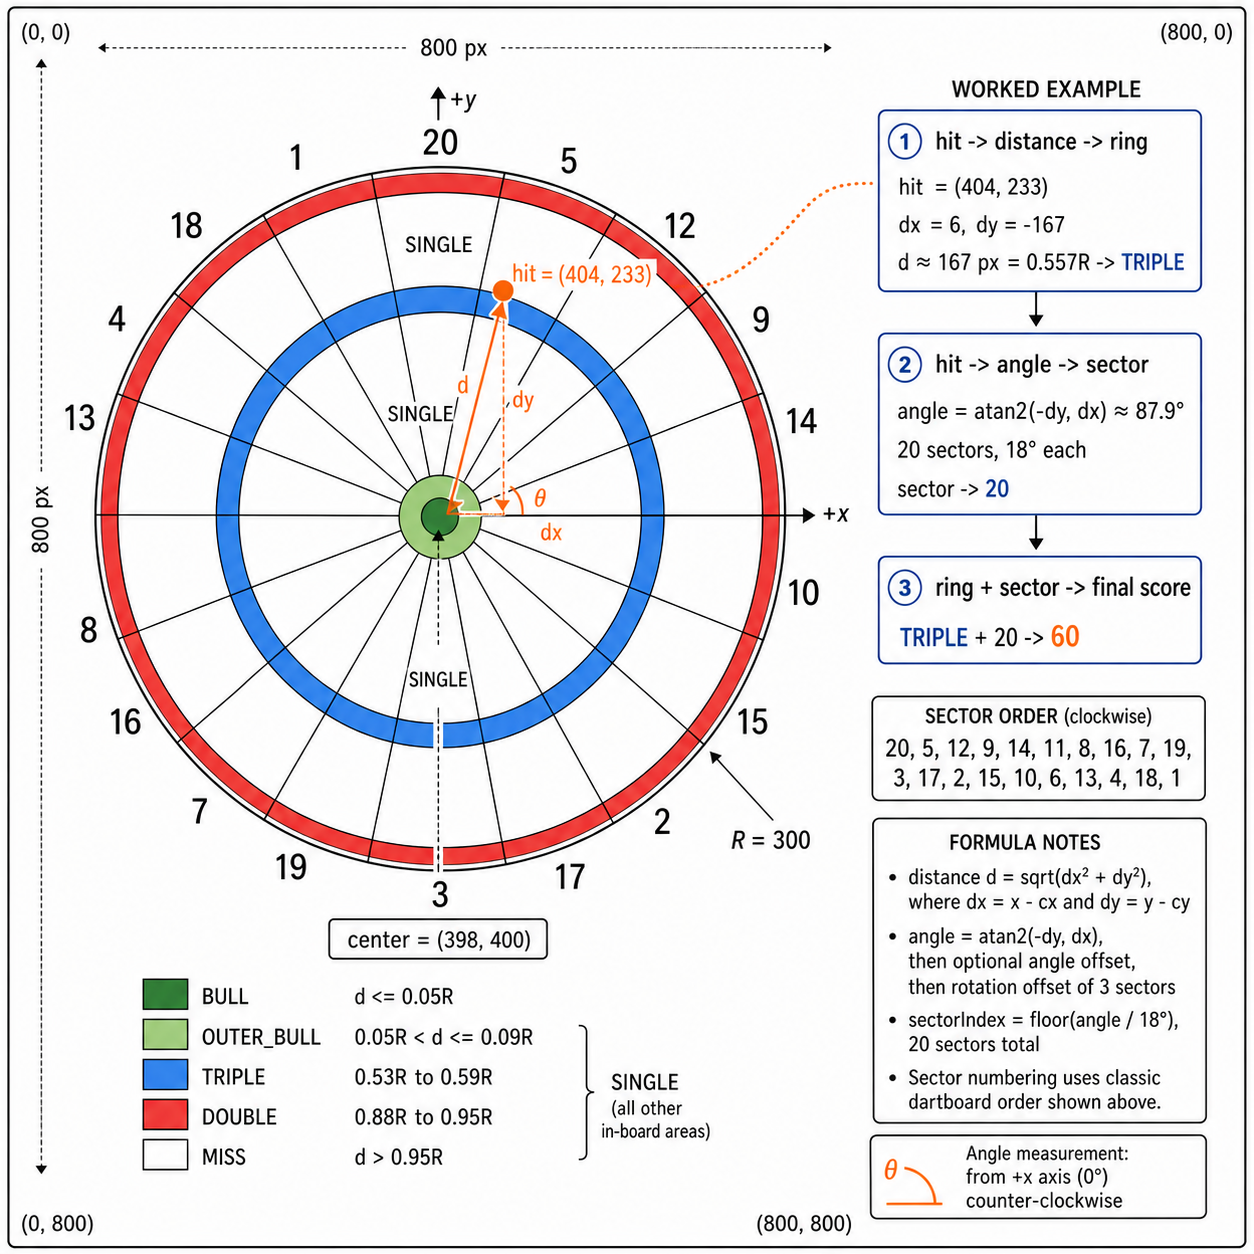
\includegraphics[width=15.5cm,keepaspectratio]{DigramDartCount.png}
\end{center}

\clearpage
\docsection{Uživatelské rozhraní}

Dotykový LCD displej slouží jako jednoduché lokální rozhraní. Zobrazuje:

\begin{itemize}
\item aktuální skóre obou hráčů
\item jednotlivé šipky v právě hraném tahu
\item součet bodů v tahu
\item stav přepnutí na dalšího hráče
\end{itemize}

Ukázky displeje:

\begin{center}
\includegraphics[width=5.25cm,keepaspectratio]{ScoreDisplay.jpeg}
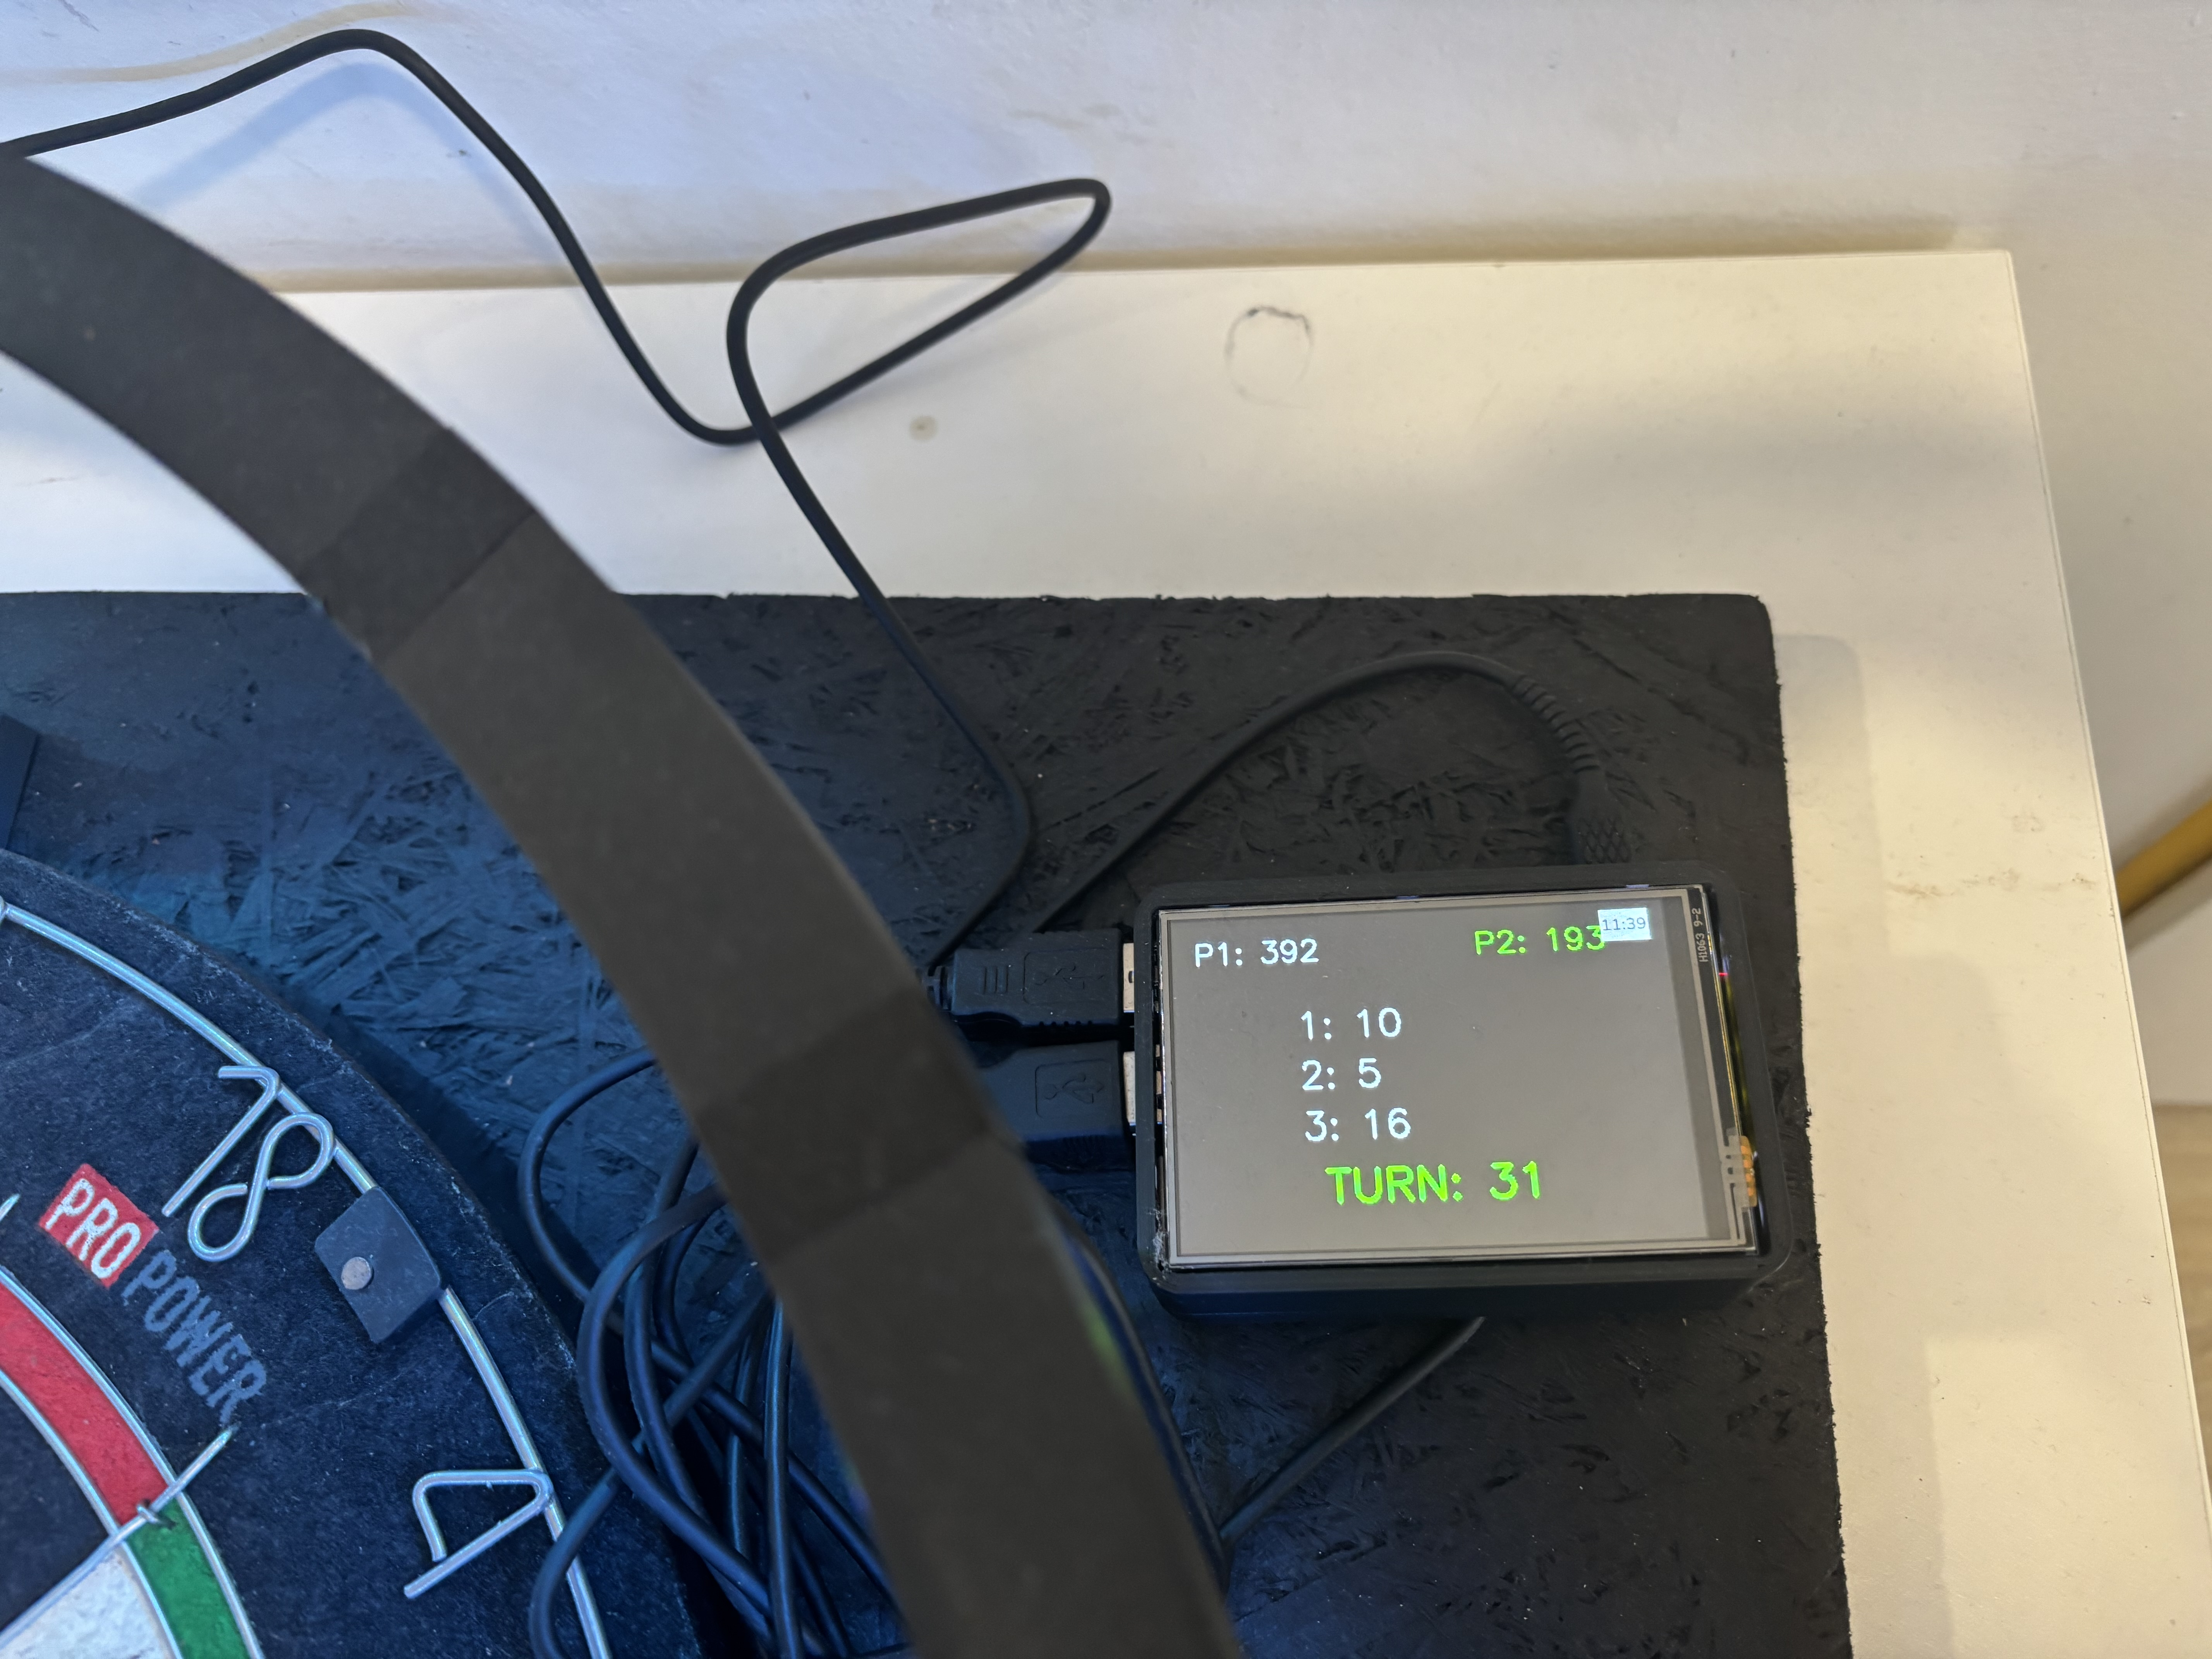
\includegraphics[width=5.25cm,keepaspectratio]{ScoredDisplay.jpeg}
\includegraphics[width=5.25cm,keepaspectratio]{DisplayNextPlayer.jpeg}
\end{center}

Při přechodu na dalšího hráče je provedena rekalibrace referenčního snímku a displej zobrazí informační obrazovku.

Ukázka celé sestavy během aktivního tahu:

\begin{center}
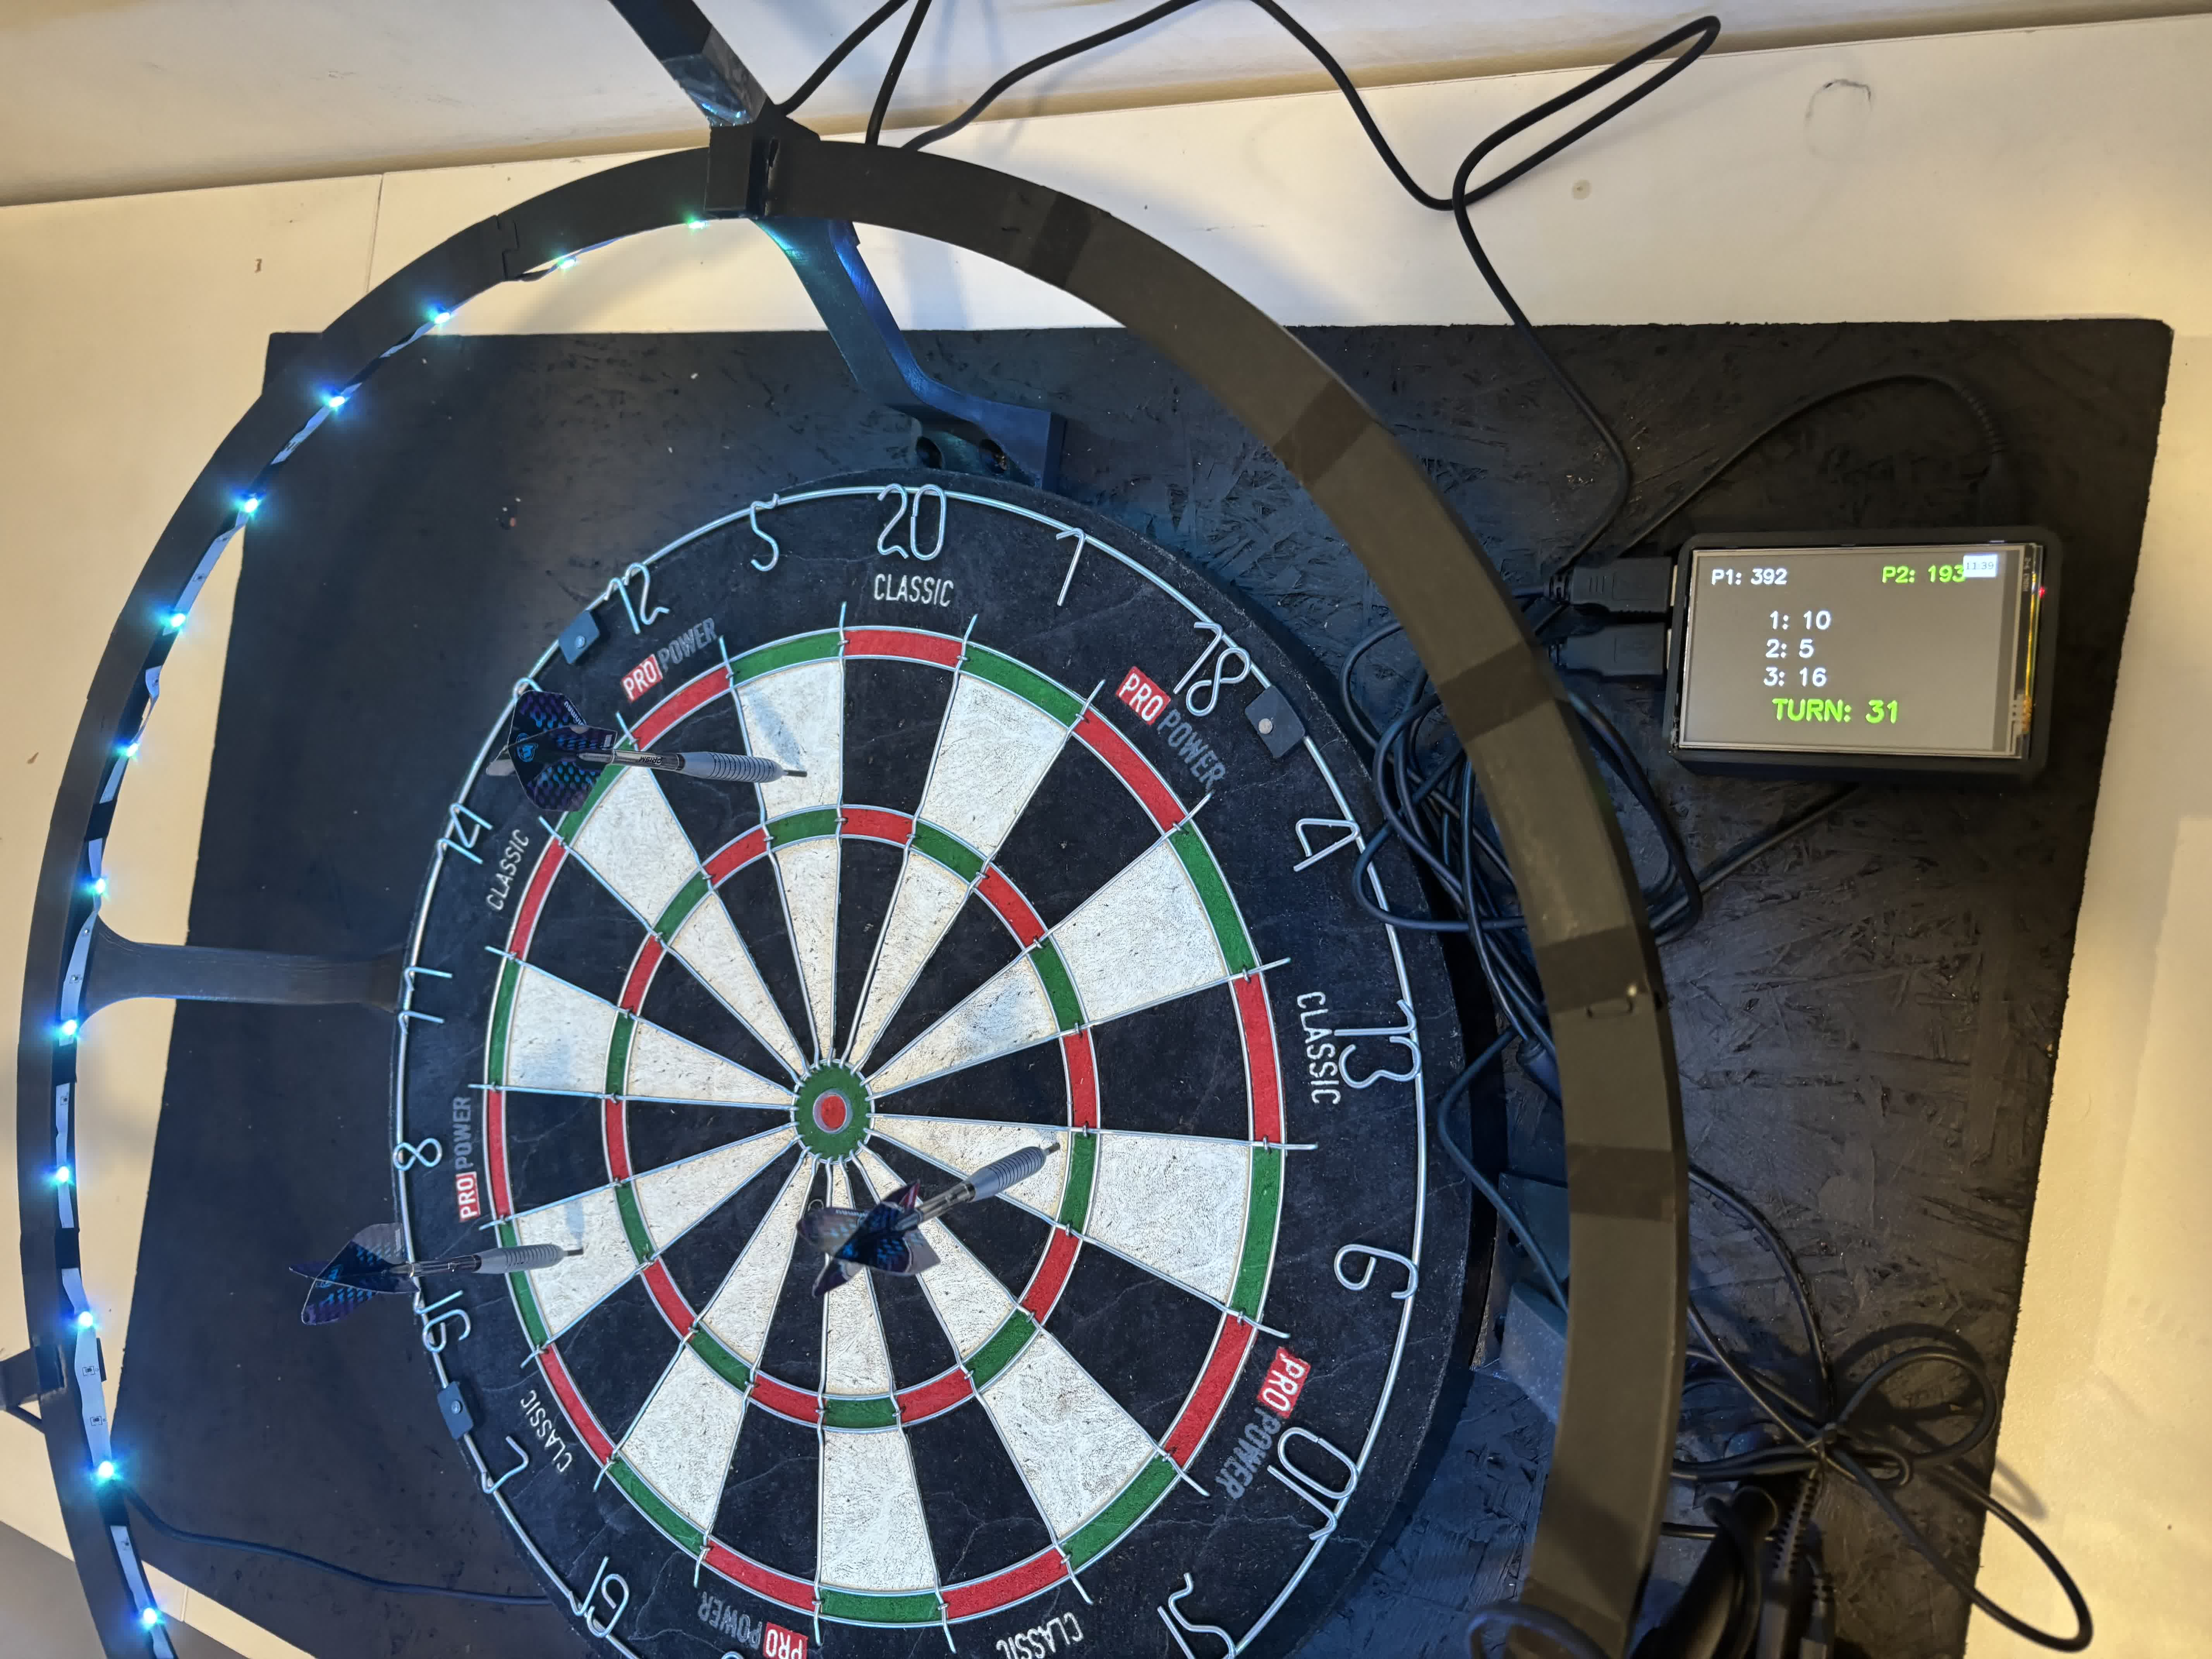
\includegraphics[width=15.5cm,keepaspectratio]{TargetScoredHorizontal.jpeg}
\end{center}

\docsection{Běh aplikace}

Aplikaci lze spustit příkazem:

\begin{verbatim}
python3 main.py
\end{verbatim}

Při správném zapojení zařízení aplikace:

\begin{itemize}
\item inicializuje kameru
\item vytvoří referenční snímek \texttt{frame.jpg}
\item spustí MJPEG server na portu \texttt{8888}
\item začne vyhodnocovat zásahy
\end{itemize}

Náhled zpracovaného videa je dostupný na adrese:

\begin{verbatim}
http://<device-ip>:8888/stream
\end{verbatim}

Ukázka celé fyzické sestavy:

\begin{center}
\includegraphics[width=\linewidth,keepaspectratio]{WholeSystem.jpeg}
\end{center}

\clearpage
\docsection{Funkční vlastnosti a omezení}

Aktuální jednokamerová verze umí:

\begin{itemize}
\item automaticky detekovat nové zásahy na základě rozdílu snímků
\item určit přibližnou špičku šipky
\item převést zásah do normalizovaného modelu terče
\item vypočítat skóre a zobrazit ho na displeji
\item přepínat hráče pomocí dotykového vstupu
\end{itemize}

Současně má několik omezení:

\begin{itemize}
\item citlivost na změny osvětlení
\item možnost falešných detekcí při pohybu ruky nebo stínech
\item starší jednokamerová architektura
\item neimplementuje pokročilá pravidla, například bust nebo double-out
\end{itemize}

\docsection{Využití AI v projektu}

Technické diagramy použité v této dokumentaci byly vytvořeny s pomocí generativní AI na základě textových promptů a následně vybrány a zasazeny do dokumentace tak, aby odpovídaly skutečné implementaci projektu. Přehled použitých promptů je uložen v souboru \texttt{AIPrompts.txt}.

\docsection{Závěr}

Využití jedné kamery se ukázalo jako dostatečné řešení pro demonstraci funkcionality a vytvoření funkčního prototypu. Výsledný systém dokáže správně určit přibližně 70 až 80 \% hozených šipek. Hlavní problémy představují proměnlivé osvětlení a překrývání jednotlivých šipek.

Z pohledu použité výpočetní platformy se zároveň ukazuje, že Raspberry Pi 4B je pro současnou jednokamerovou implementaci s USB kamerou Canyon CWC3 do určité míry kanón na vrabce. Prototyp na této platformě bez problémů běží a poskytuje dostatečnou rezervu pro vývoj i ladění, ale samotná úloha založená na jedné kameře a klasickém zpracování obrazu nevyužívá plný potenciál takto výkonného zařízení. To je důležité i z hlediska budoucí optimalizace, protože po zpřesnění algoritmů a stabilizaci celé pipeline bude možné uvažovat o nasazení na úspornější a levnější hardware.

Projekt bude dále sloužit jako základ pro automatickou anotaci snímků hozených šipek. Takto anotovaná data budou následně využita pro natrénování neuronové sítě s využitím modelu YOLO. Tento přístup by mohl přinést přesnější odhad pozice šipky, lepší responzivitu systému a případně i snížení výpočetních nároků.

\clearpage
\docsection{Bibliografie}

\begin{enumerate}
\item WAVESHARE. \textit{3.5inch RPi LCD (B)} [online]. Waveshare Wiki. [cit. 2026-05-01]. Dostupné z: \url{https://www.waveshare.com/wiki/3.5inch_RPi_LCD_%28B%29}

\item RASPBERRY PI LTD. \textit{Configuration - Raspberry Pi Documentation} [online]. Raspberry Pi Documentation. [cit. 2026-05-01]. Dostupné z: \url{https://www.raspberrypi.com/documentation/configuration/web-interface/raspberry-pi.html}

\item REDMON, Joseph, SANTOSH DIVVALA, ROSS GIRSHICK a ALI FARHADI. \textit{You Only Look Once: Unified, Real-Time Object Detection} [online]. arXiv, 2016. DOI: \url{https://doi.org/10.48550/arXiv.1506.02640}. [cit. 2026-05-01]. Dostupné z: \url{https://arxiv.org/abs/1506.02640}

\item ULTRALYTICS. \textit{Ultralytics YOLO Docs} [online]. Ultralytics Documentation. [cit. 2026-05-01]. Dostupné z: \url{https://docs.ultralytics.com/}

\item OPENCV. \textit{Geometric Transformations of Images} [online]. OpenCV Documentation. [cit. 2026-05-01]. Dostupné z: \url{https://docs.opencv.org/4.x/da/d6e/tutorial_py_geometric_transformations.html}

\item OPENCV. \textit{Geometric Image Transformations} [online]. OpenCV Documentation. [cit. 2026-05-01]. Dostupné z: \url{https://docs.opencv.org/4.x/da/d54/group__imgproc__transform.html}

\item OPENCV. \textit{Contours: Getting Started} [online]. OpenCV Documentation. [cit. 2026-05-01]. Dostupné z: \url{https://docs.opencv.org/3.4/d4/d73/tutorial_py_contours_begin.html}
\end{enumerate}

\end{document}
